\chapter{Tecnologie Impiegate}
\label{chap:tecnologie}

Il progetto ICOS utilizza diverse tecnologie del web semantico per la gestione dei dati e dei metadati relativi alle misurazioni dell'anidride carbonica e di altri gas serra effettuate dalle stazioni di monitoraggio ICOS. Alcune delle principali tecnologie utilizzate sono:

\section{RDF}
\label{section:rdf}
RDF (Resource Description Framework): il progetto ICOS utilizza il
formato RDF per rappresentare i dati e i metadati relativi
alle misurazioni delle stazioni di monitoraggio.
RDF è un formato standard del web semantico utilizzato
per rappresentare le informazioni in modo strutturato.\\

In particolare ICOS utilizza sia la sintassi RDF/XML sia quella
RDF/Turtle, lasciando la possibilità all'utente di scaricare i dati
nel formato che preferiscono.

\section{OWL}
\label{section:owl}
OWL (Web Ontology Language): l'ontologia ICOS
Carbon Portal utilizza il linguaggio formale OWL
per definire i concetti e le relazioni tra i concetti.
OWL è un linguaggio standard del web semantico utilizzato
per descrivere ontologie e sviluppato dal W3C come estensione
del linguaggio RDF.\\

ICOS ha definito un vocabolario OWL per la
descrizione dei metadati dei dati raccolti
dalle stazioni di monitoraggio ICOS,
in particolare per quanto riguarda la struttura,
la qualità e le informazioni sul contesto di
acquisizione dei dati. Questa particolare ontologia non solo
viene usata da ICOS ma anche da SITES (Swedish
Infrastructure for Ecosystem Science) \cite{SITESHomepage},
l'infrastruttura nazionale svedese per la ricerca sul campo
terrestre e limnologica.

\section{SPARQL}
\label{section:sparql}
SPARQL (SPARQL Protocol and RDF Query Language): il progetto
ICOS utilizza SPARQL per interrogare e recuperare i dati e
i metadati delle stazioni di monitoraggio.
SPARQL è un linguaggio di interrogazione standard
del web semantico utilizzato per recuperare informazioni
dalle ontologie RDF.\\

Inoltre, ICOS fornisce un endpoint SPARQL pubblico,
che consente agli utenti di eseguire query SPARQL sui dati
e metadati ICOS. L'interfaccia, come si può notare in figura \ref{figure:sparqlendpoint}, permette di scrivere query personalizzate
oppure selezionarne una pre-esistente. Infine, si può liberamente
scegliere il formato del risultato ritornato dalla richiesta tra JSON,
CSV, XML e Turtle.

\begin{figure}[h!]
    \centering
    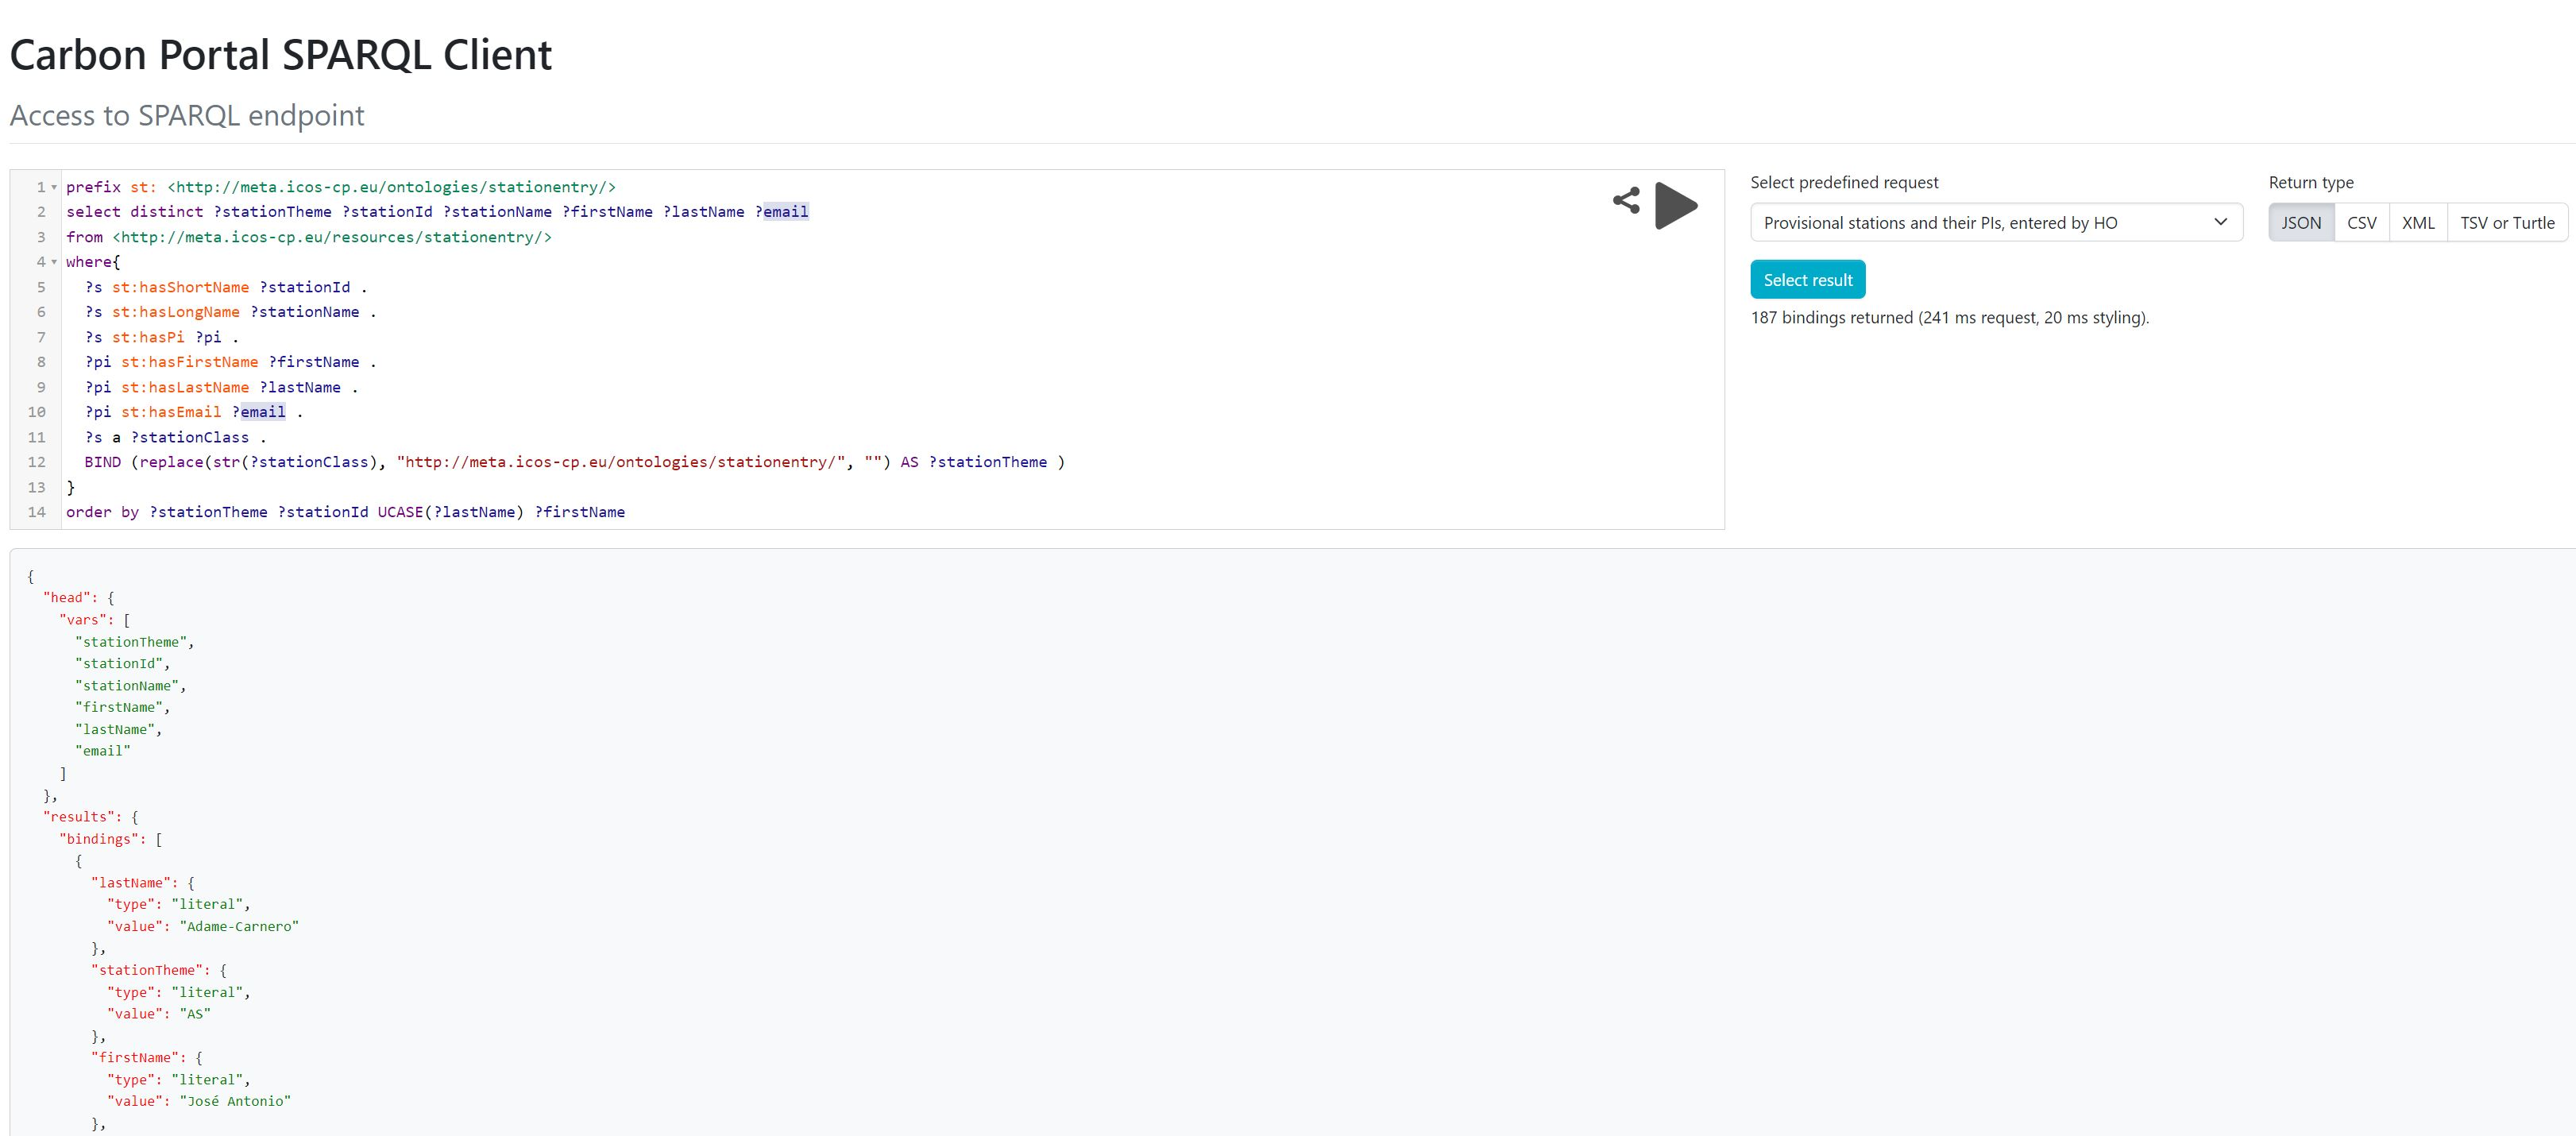
\includegraphics[width=0.8\textwidth]{figures/sparqlendpoint.JPG}
    \caption{L'endpoint SPARQL di ICOS con una query d'esempio eseguita.}
    \label{figure:sparqlendpoint}
\end{figure}

\section{Jupyter}
\label{section:jupyter}
Jupyter è un ambiente di lavoro interattivo per la creazione e condivisione di documenti che contengono codice, testo, visualizzazioni e altri elementi multimediali.
ICOS utilizza Jupyter come uno strumento fondamentale per l'analisi e la visualizzazione dei dati raccolti dalle stazioni di monitoraggio ICOS.\\

Per facilitare agli utenti l'accesso,
l'elaborazione e l'interazione con i
dati ICOS, ICOS Carbon Portal
offre diverse soluzioni tramite Jupyter \cite{JupyterICOS}.
Esistono soluzioni pre-implementate, 
che consentono la collaborazione tra
scienziati che lavorano allo
stesso progetto, condividendo dati
e codice. Inoltre, esistono soluzioni
per rispondere alle esigenze degli
scienziati che desiderano utilizzare
i dati ICOS in combinazione con
i propri dati. Infine, ICOS
Carbon Portal ha sviluppato
notebook Jupyter specifici per promuovere i dati,
i metadati e il ruolo di ICOS a
persone che potrebbero non avere
alcun collegamento diretto o
conoscenza preliminare di ICOS,
come ricercatori, responsabili politici,
educatori, studenti o persone di ogni tipo.

\section{Linked Data}
\label{section:linkeddata}
Il progetto ICOS segue il principio di Linked Data, tecnologia moderna
e avanzata nel campo della gestione dati, che consente di distribuire
i dati tramite collegamenti Internet (creazione di link tra
le risorse RDF), sui quali l'utente
può semplicemente fare clic per visualizzare
e/o scaricare i dati. Ciò consente di creare
una rete di dati interconnessi
e di aumentare la loro interoperabilità. 
Inoltre, rende possibile la \textit{machine-to-machine
communication}, 
che rappresenta lo scambio di informazioni (prevalentemente
automatico,
quindi senza intervento umano) tra dispositivi di varia natura 
oppure mediante un sistema di elaborazione dati centrale.



